\documentclass{article}
\usepackage{amsmath}
\usepackage{graphicx}
\usepackage{listings}
\usepackage{hyperref}

\title{Parziale Progettazione di Sistemi Elettronici 14/11/24}
\author{Marco Losso}
\date{\today}

\begin{document}

\maketitle

\section{Introduzione}
Questo report descrive il progetto di un cronometro sviluppato in Verilog.
Il cronometro conta secondi, decimi e centesimi di secondo e include funzionalità come il reset, il start/stop, la visualizzazione del tempo parziale e il conteggio alla rovescia.
Inoltre, sono state implementate funzioni per contare i minuti e le ore e per commutare tra diverse modalità di visualizzazione.

Il progetto Verilog è stato simulato utilizzando ModelSim e infine caricato sulla scheda DE1-SoC di Terasic per apprezzarne il risultato finale sui sei display a sette segmenti presenti su di essa.


\section{Descrizione del Cronometro}
Il cronometro di base è stato progettato per contare secondi, decimi e centesimi di secondo. 
Sono stati implementati due tasti principali: \textbf{reset} e \textbf{start/stop}. 
Il tasto di reset azzera il conteggio, mentre il tasto di start/stop permette di avviare e fermare il conteggio. 
Nel momento in cui il cronometro viene resettato, rimane fermo sul valore zero fino a quando il tasto di start/stop non viene premuto nuovamente per avviare il conteggio.

\section{Clock Divider}

Il progetto utilizza un \textbf{clock divider} per generare un segnale di clock a 100 Hz partendo da un segnale a 50 MHz interno alla scheda De1-SoC. 
Questo assicura una frequenza di aggiornamento adeguata per il conteggio dei centesimi di secondo. 
Ciò viene implementato tramite il conteggio del numero di fronti di salita del clock a 50 MHz, pari a 500.000 in 0.01 secondi: quindi 250.000 per il fronte alto e altrettanti per il fronte basso.
Al termine del conteggio il valore del clock a 100 Hz in uscita viene negato per generare, appunto, i due stati alto e basso. 
Di seguito viene riportato per intero il modulo che implementa il \textbf{clock divider} ed è facile riconoscere le operazioni appena descritte.

\begin{lstlisting}[language=Verilog, caption={Clock Divider}]
module clock_divider (
    input clk_in,    // Clock a 50 MHz
    output reg clk_out   // Clock a 100 Hz
);
    reg [18:0] counter;
    initial begin
        counter = 0;
        clk_out = 0;
    end

    always @(posedge clk_in) begin
        if (counter == 250000) begin
            counter <= 0;
            clk_out <= ~clk_out;
        end else begin
            counter <= counter + 1;
        end
    end
endmodule
\end{lstlisting}

\subsection{Descrizione delle Variabili} 

\begin{itemize} 
    \item \textbf{clk\_in}: Segnale di clock in ingresso a 50 MHz.
    \item \textbf{clk\_out}: Segnale di clock in uscita a 100 Hz.
    \item \textbf{counter}: Contatore che tiene traccia dei cicli di clock per generare il clock in uscita.
\end{itemize}

\newpage

\section{Contatore}

Successivamente si è passati alla realizzazione del conteggio vero e proprio, il tutto è stato realizzato con degli \texttt{if} annidati che introducono anche il conteggio dei minuti e delle ore.

Di seguito è stato riportato solo un estratto del modulo che implementa il \textbf{contatore} mettendo in luce proprio la struttura degli \texttt{if}. Inoltre, si evidenzia come all'attivarsi del \texttt{reset} questo pone il valore del conteggio a 0, e l'utilizzo dell'\texttt{enable} per fermare o far ripartire il conteggio implementando la funzione di start/stop.

\begin{lstlisting}[language=Verilog, caption={Estratto del Modulo del Contatore}]
always @(posedge clk_100Hz or posedge rst) begin
    if (rst) begin
        // Reset del conteggio
        centisec <= 0;
        sec <= 0;
        min <= 0;
        hr <= 0;
        running <= 0;
    end else begin
        if (enable && !enable_reg) begin
            running <= ~running; // Cambia lo stato del contatore
        end
        enable_reg <= enable; // Aggiorna lo stato del tasto enable
        if (running) begin
            if (centisec == 99) begin
                centisec <= 0;
                if (sec == 59) begin
                    sec <= 0;
                    if (min == 59) begin
                        min <= 0;
                        if (hr == 23)
                            hr <= 0;
                        else
                            hr <= hr + 1;
                    end else
                        min <= min + 1;
                end else
                    sec <= sec + 1;
            end else
                centisec <= centisec + 1;
        end
    end
end
\end{lstlisting}

\subsection{Descrizione delle Variabili}
\begin{itemize}
    \item \textbf{centisec}: Contatore dei centesimi di secondo.
    \item \textbf{sec}: Contatore dei secondi.
    \item \textbf{min}: Contatore dei minuti.
    \item \textbf{hr}: Contatore delle ore.
    \item \textbf{running}: Stato del contatore (avviato/arrestato).
    \item \textbf{enable\_reg}: Registrazione dello stato precedente del tasto enable.
\end{itemize}

\subsection{Prima simulazione}

Prima di procedere al download su scheda è stata eseguita una simulazione di questa prima parte di progetto su Modelsim in modo da verificare il corretto funzionamento del contatore e anche dei segnali di \texttt{reset} e \texttt{enable}.

La figura sottostante mostra i risulatati della simualzione e soprattutto come i segnali di \texttt{reset} e \texttt{enable} interagiscano con il contatore.

\vspace{1em}

\begin{figure}[!ht]
    \centering
    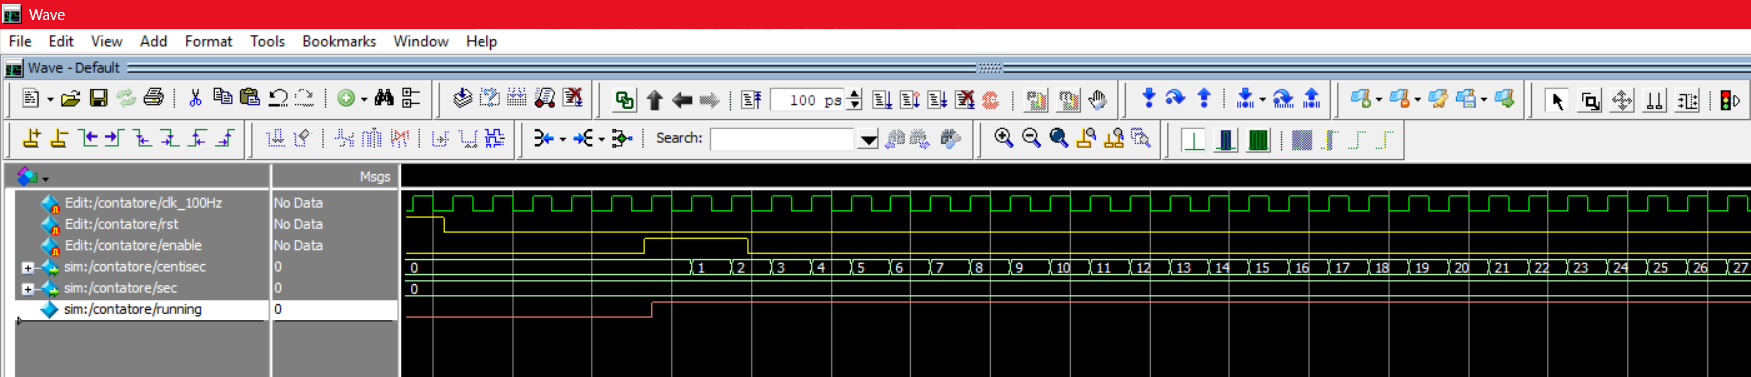
\includegraphics[width=\linewidth]{Immagini/Simulazione_Contatore.png}
    \caption{Simulazione contatore in ModelSim}
    \label{fig: Simulazione_Contatore}
\end{figure}

\newpage

\section{Implementazione dei Tempi Parziali}
La funzionalità di visualizzazione del tempo parziale è stata aggiunta utilizzando un tasto dedicato. Quando il tasto di tempo parziale viene premuto, i valori attuali del cronometro vengono congelati e visualizzati sui display a 7 segmenti per 5 secondi, senza interrompere il conteggio reale. Questo consente di visualizzare il tempo parziale in qualsiasi momento, mantenendo il cronometro in esecuzione.

L'estratto di codice Verilog seguente mostra come i valori del cronometro vengono memorizzati e visualizzati per 5 secondi quando il tasto di tempo parziale viene premuto:

\begin{lstlisting}[language=Verilog, caption={Gestione del Tempo Parziale}]
always @(posedge clk) begin
    if (parziale_mode) begin
        if (parziale_counter < 500) begin // 5 secondi a 100 Hz
            parziale_counter <= parziale_counter + 1;
        end else begin
            parziale_mode <= 0;
            parziale_counter <= 0;
        end
    end

    if (parziale && !parziale_mode) begin
        // Attiva la visualizzazione del tempo parziale 
        // quando il tasto e' premuto
        parziale_mode <= 1;
        parziale_counter <= 0;
        // Memorizza i valori attuali del contatore
        parziale_centisec <= centisec;
        parziale_sec <= sec;
        parziale_min <= min;
        parziale_hr <= hr;
    end
end
\end{lstlisting}

\subsection{Descrizione delle Variabili}
\begin{itemize}
    \item \textbf{parziale\_mode}: Stato del tempo parziale.
    \item \textbf{parziale\_counter}: Contatore che tiene traccia del tempo di visualizzazione del tempo parziale.
    \item \textbf{parziale\_centisec}, \textbf{parziale\_sec}, \textbf{parziale\_min}, \textbf{parziale\_hr}: Memorizzano i valori correnti del cronometro quando il tasto di tempo parziale viene premuto.
\end{itemize}

\newpage

\section{Implementazione del Conteggio all'Indietro}
È stata aggiunta una funzionalità per consentire al cronometro di contare all'indietro utilizzando uno switch dedicato. 
Quando lo switch è attivato, il cronometro conta all'indietro; quando lo switch è disattivato, il cronometro conta in avanti.

\subsection{Codice Verilog per il Conteggio all'Indietro}
L'estratto di codice Verilog seguente mostra come il conteggio viene gestito all'indietro in base allo stato dello switch:

\begin{lstlisting}[language=Verilog, caption={Gestione del Conteggio all'Indietro}]
if (direction) begin
    // Conteggio inverso
    if (centisec == 0) begin
        centisec <= 99;
        if (sec == 0) begin
            sec <= 59;
            if (min == 0) begin
                min <= 59;
                if (hr == 0)
                    hr <= 23;
                else
                    hr <= hr - 1;
            end else
                min <= min - 1;
        end else
            sec <= sec - 1;
    end else
        centisec <= centisec - 1;
end
\end{lstlisting}

\subsection{Descrizione delle Variabili}
\begin{itemize}
    \item \textbf{direction}: Switch che determina la direzione del conteggio (0 = avanti, 1 = indietro).
    \item \textbf{centisec}, \textbf{sec}, \textbf{min}, \textbf{hr}: Variabili che memorizzano i valori del conteggio del cronometro.
\end{itemize}

\newpage

\section{Simulazione Finale del Progetto}
La simulazione finale del progetto è stata implementata in un modulo top entity che include l'utilizzo dei tasti e degli switch veri e propri. Questo ha permesso di testare il comportamento del sistema in condizioni realistiche, utilizzando input fisici per controllare il funzionamento del contatore e la visualizzazione sui display a 7 segmenti.

I valori del contatore sono stati convertiti in BCD (Binary-Coded Decimal) per poter essere visualizzati correttamente sui display a 7 segmenti.

\subsection{Descrizione dei Segnali Utilizzati}
Nella simulazione finale, sono stati utilizzati vari segnali e bus per controllare il funzionamento del sistema:
\begin{itemize}
    \item \textbf{CLOCK\_50}: Segnale di clock a 50 MHz.
    \item \textbf{clk\_100Hz}: Segnale di clock a 100 Hz generato dal clock divider.
    \item \textbf{KEY[0]}: Tasto di reset.
    \item \textbf{KEY[1]}: Tasto di enable per avviare e fermare il conteggio.
    \item \textbf{KEY[2]}: Tasto di tempo parziale per fermare la visualizzazione nei display a 7 segmenti.
    \item \textbf{HEX}: Bus per i display a 7 segmenti.
    \item \textbf{disp}: Segnale che controlla i display a 7 segmenti.
    \item \textbf{sec, centisec, min}: Variabili che memorizzano i valori del contatore.
\end{itemize}

\subsection{Risultati della Simulazione}
Le seguenti immagini mostrano i risultati della simulazione:

\begin{itemize}
    \item Nella figura \ref{fig:simulazione1}, oltre al tasto di reset KEY[0] utilizzato all'inizio, si vede l'impiego dell'enable KEY[1] che ferma il conteggio sia del contatore (linee gialle), sia quello raffigurato nei display a 7 segmenti (linee rosa).
    \item Nella figura \ref{fig:simulazione2} viene impiegato il tasto parziale \texttt{KEY[2]} che ferma solo la visualizzazione nei display a 7 segmenti (linee rosa) ma il conteggio del contatore prosegue (linee gialle).
\end{itemize}

\newpage

\begin{figure}[!ht]
    \centering
    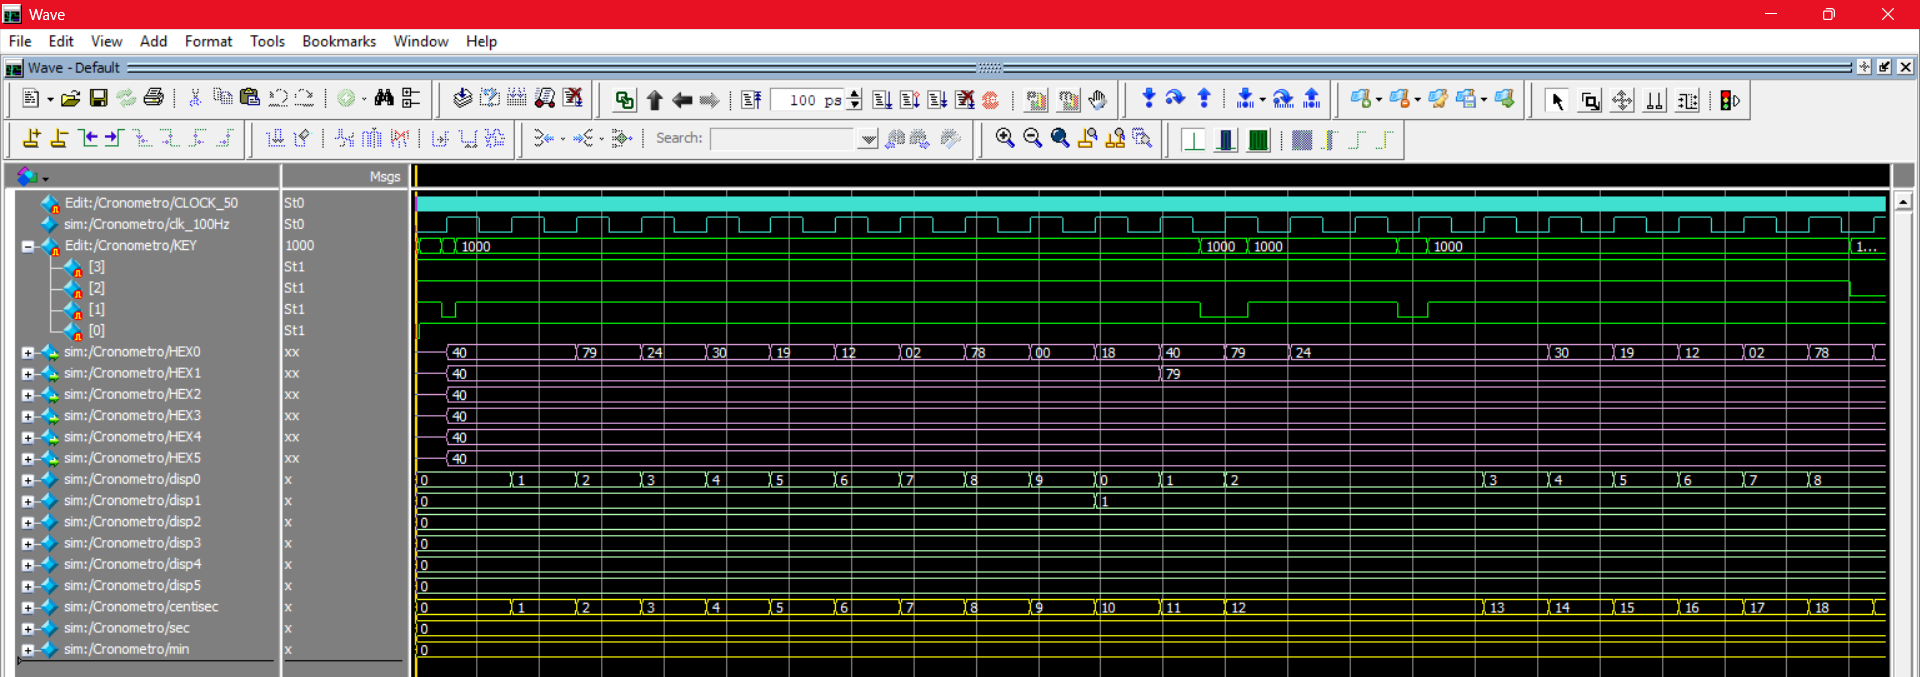
\includegraphics[width=\textwidth]{Immagini/Simualzione_Finale_1.png}
    \caption{Simulazione che mostra l'impiego del tasto di reset (KEY[0]) e del tasto di enable (KEY[1]) per fermare il conteggio.}
    \label{fig:simulazione1}
\end{figure}


\begin{figure}[!ht]
    \centering
    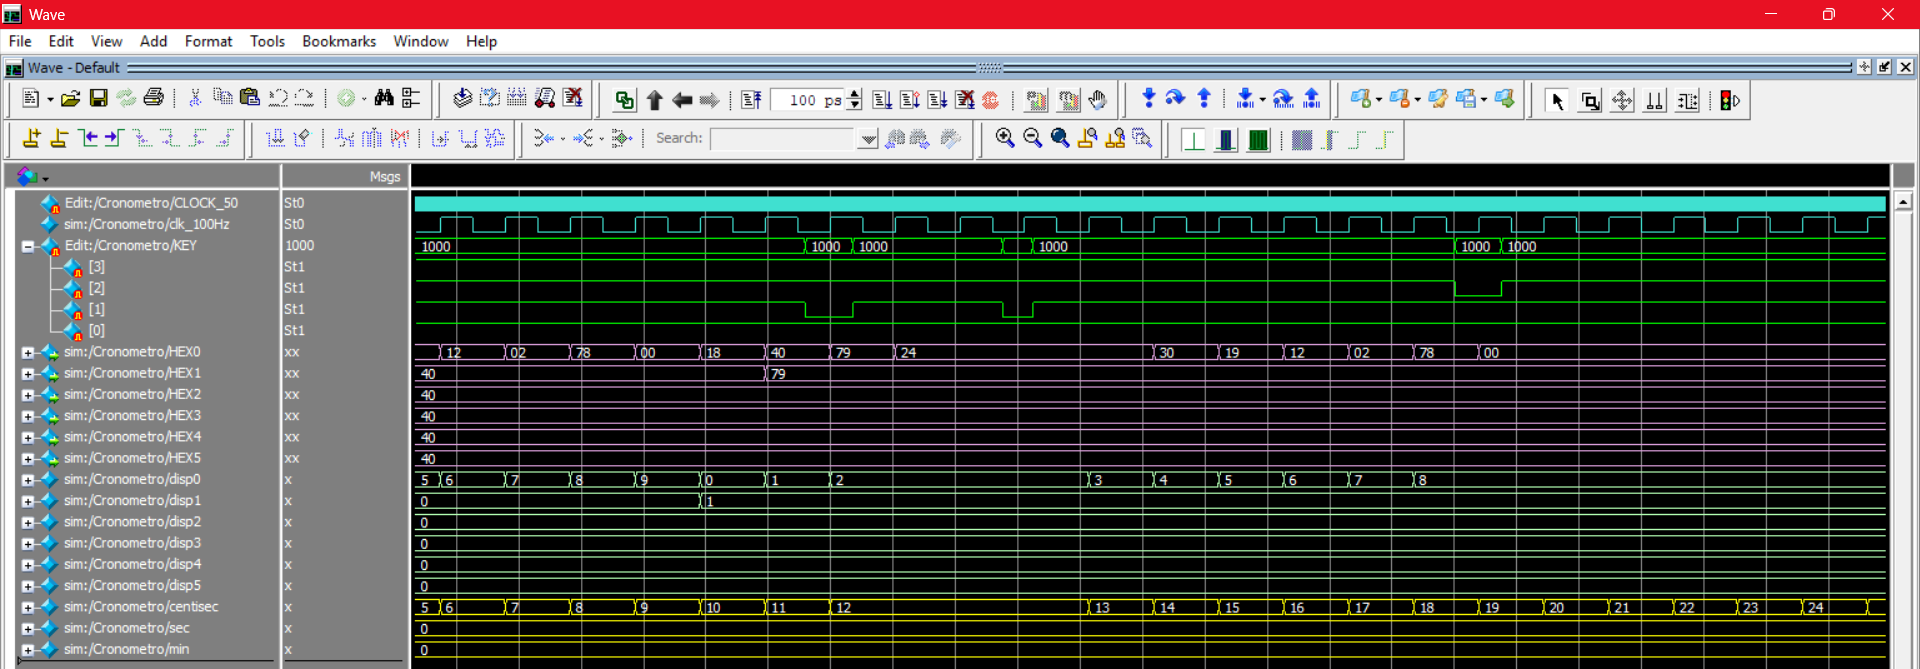
\includegraphics[width=\textwidth]{Immagini/Simualzione_Finale_2.png}
    \caption{Simulazione che mostra l'utilizzo del tasto parziale (KEY[2]) per fermare solo la visualizzazione nei display a 7 segmenti (linee rosa), mentre il conteggio del contatore prosegue (linee gialle).}
    \label{fig:simulazione2}
\end{figure}

\newpage

\section{Modalità di Visualizzazione nei Display a 7 Segmenti}
Dato che sono disponibili solo 6 display a 7 segmenti, è stata implementata una funzionalità che consente di passare tra due modalità di visualizzazione utilizzando il tasto KEY[3]. Questo tasto permette di switchare dalla visualizzazione dei centesimi di secondo, secondi e minuti (\textbf{centisec-sec-min}) a quella dei secondi, minuti e ore (\textbf{sec-min-hr}).

\subsection{Codice Verilog per le Modalità di Visualizzazione}
Di seguito è riportato un estratto del codice Verilog che gestisce le modalità di visualizzazione nei display a 7 segmenti:

\begin{lstlisting}[language=Verilog, caption={Gestione delle Modalità di Visualizzazione}]
always @(posedge clk) begin
    if (key3) begin
        mode <= ~mode; 
        // Cambia modalita' quando KEY[3] e' premuto
    end
end

always @(*) begin
    if (mode == 0) begin
        // Visualizza centisec-sec-min
        disp0 = centisec % 10;
        disp1 = centisec / 10;
        disp2 = sec % 10;
        disp3 = sec / 10;
        disp4 = min % 10;
        disp5 = min / 10;
    end else begin
        // Visualizza sec-min-hr
        disp0 = sec % 10;
        disp1 = sec / 10;
        disp2 = min % 10;
        disp3 = min / 10;
        disp4 = hr % 10;
        disp5 = hr / 10;
    end
end
\end{lstlisting}

\newpage

La divisione per 10 viene fatta per convertire i valori in formato BCD (Binary-Coded Decimal). Nei display a 7 segmenti, i numeri devono essere visualizzati cifra per cifra in formato decimale. La divisione per 10 permette di separare le unità dalle decine per ogni valore da visualizzare, rendendo possibile mostrare ogni cifra individualmente su ciascun display.

\subsection{Descrizione delle Variabili}
\begin{itemize}
    \item \textbf{key3}: Tasto utilizzato per cambiare modalità di visualizzazione.
    \item \textbf{mode}: Variabile che determina la modalità di visualizzazione (0 = centisec-sec-min, 1 = sec-min-hr).
    \item \textbf{disp0, disp1, disp2, disp3, disp4, disp5}: Variabili che controllano i display a 7 segmenti.
    \item \textbf{centisec, sec, min, hr}: Variabili che memorizzano i valori del conteggio.
\end{itemize}

\newpage

\section{Conclusioni}

Il progetto sviluppato in Quartus ha raggiunto con successo l'obiettivo di creare un cronometro utilizzando Verilog. Le funzionalità implementate includono il conteggio dei centesimi di secondo, secondi, minuti e ore, l'uso di tasti per il reset e lo start/stop, la visualizzazione del tempo parziale, il conteggio all'indietro e la commutazione tra diverse modalità di visualizzazione sui display a 7 segmenti.

La simulazione finale del progetto è stata condotta utilizzando ModelSim, e l'implementazione è stata verificata sulla scheda DE1-SoC di Terasic. Sono stati effettuati tutti i test necessari sulla scheda hardware e il sistema ha funzionato perfettamente in ogni sua parte. Questo ha permesso di validare il funzionamento del cronometro in un ambiente realistico, garantendo che tutte le funzionalità operino correttamente.

Attraverso questo progetto, sono state acquisite essenziali competenze nella progettazione hardware utilizzando Verilog, nella simulazione di sistemi digitali e nell'integrazione di componenti hardware e software. La capacità di gestire segnali di clock, implementare logiche di conteggio e visualizzare dati su display a 7 segmenti sono state abilità cruciali sviluppate durante il corso del progetto.

Il successo del progetto apre la strada a potenziali miglioramenti futuri, come l'aggiunta di ulteriori modalità di conteggio, l'integrazione con altri dispositivi esterni e l'ottimizzazione delle prestazioni.

Questi miglioramenti potrebbero ulteriormente ampliare le capacità e le applicazioni del cronometro sviluppato.

\end{document}